% !TEX root = SystemTemplate.tex

\chapter{Overview and concept of operations}

The overview should take the form of an executive summary. Give the reader a feel for the purpose of the document, what is contained in the document, and an idea of the purpose for the system or product.


\section{Scope}
This document covers the design and implementation of the program.

\section{Purpose}
The purpose of this program is to assign pass/fail grades to simple programs run against a number of test cases. 

\subsection{Compilation}
In order to test a program, it must be compiled into an executable.

\subsection{Directory Crawl}
This component finds all of the test cases. 

\subsection{Test Execution}
The target program will be executed against a number of test cases.

\subsection{Result Logging}
Results of the tests must be recorded for the user to read.

\section{Systems Goals}
The goal of this system is to perform automated testing and grading for C++ programs.

\section{System Overview and Diagram}
The program begins by finding all test files. Then, the target program is compiled. Next, all of the test cases are executed. Finally, the results are written to the log file.

\begin{figure}[tbh]
\begin{center}
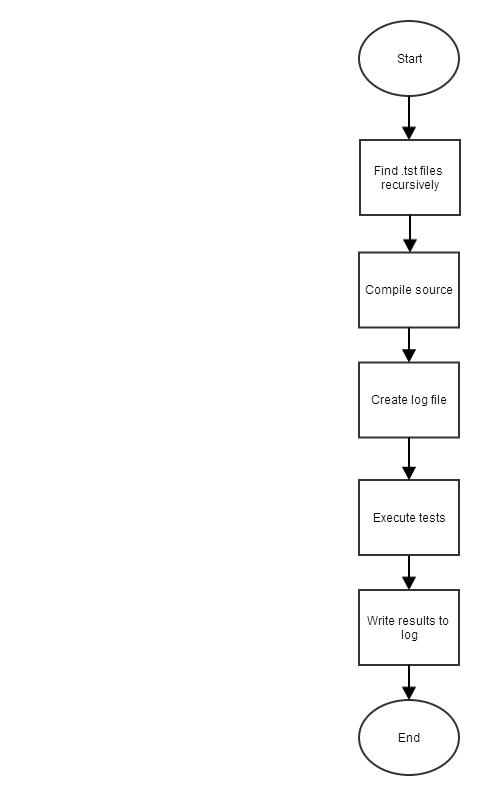
\includegraphics[width=0.75\textwidth]{./soft_eng_prog1}
\end{center}
\caption{Program flowchart \label{systemdiagram}}
\end{figure}

\section{Technologies Overview}
Developed in Linux in C++, using the g++ compiler.\newline
Documentation created using TexWorks and MikTex.\newline
Flowchart created using Gliffy.\newline

\section{Terminology and Acronyms}

See Table 1.1
\begin{table}[tbh]
\begin{center}
\begin{tabular}{|r|l|}
\hline
    GPL & General public licenced software such as GNU\textbackslash Linux environments and tools \\ \hline
    Agile Methodology & An approach to project management as it relates to software engineering \url{agilemanifesto.org} \\ \hline
    C++  STL & Standard Template Libraries: classes and methods used in common C++. \\
    \hline
\end{tabular}
\caption{Defining Some Important Terms \label{terms}}
\end{center}
\end{table}